%%%%%%%%%%%%%%%%%%%%%%%%%%%%%%%%%%%%%%%%%%%%%%%%%%%%%%%%%%%%%%%%%%%%%%%%%%%%%%%
%                       CARREGA DE LA CLASSE DE DOCUMENT                      %
%                                                                             %
% Les opcions admissibles son:                                                %
%      12pt / 11pt            (cos dels tipus de lletra; no feu servir 10pt)  %
%                                                                             %
% catalan/spanish/english     (llengua principal del treball)                 %
%                                                                             % 
% french/italian/german...    (si necessiteu fer servir alguna altra llengua) %
%                                                                             %
% listoffigures               (El document inclou un Index de figures)        %
% listoftables                (El document inclou un Index de taules)         %
% listofquadres               (El document inclou un Index de quadres)        %
% listofalgorithms            (El document inclou un Index d'algorismes)      %
%                                                                             %
%%%%%%%%%%%%%%%%%%%%%%%%%%%%%%%%%%%%%%%%%%%%%%%%%%%%%%%%%%%%%%%%%%%%%%%%%%%%%%%

\documentclass[12pt,spanish,listoffigures,listoftables]{tfgetsinf}

%%%%%%%%%%%%%%%%%%%%%%%%%%%%%%%%%%%%%%%%%%%%%%%%%%%%%%%%%%%%%%%%%%%%%%%%%%%%%%%
%                     CODIFICACIO DEL FITXER FONT                             %
%                                                                             %
%    windows fa servir normalment 'ansinew'                                   %
%    amb linux es possible que siga 'latin1' o 'latin9'                       %
%    Pero el mes recomanable es fer servir utf8 (unicode 8)                   %
%                                          (si el vostre editor ho permet)    % 
%%%%%%%%%%%%%%%%%%%%%%%%%%%%%%%%%%%%%%%%%%%%%%%%%%%%%%%%%%%%%%%%%%%%%%%%%%%%%%%

\usepackage[utf8]{inputenc} 

%%%%%%%%%%%%%%%%%%%%%%%%%%%%%%%%%%%%%%%%%%%%%%%%%%%%%%%%%%%%%%%%%%%%%%%%%%%%%%%
%                        ALTRES PAQUETS I DEFINICIONS                         %
%                                                                             %
% Carregueu aci els paquets que necessiteu i declareu les comandes i entorns  %
%                                          (aquesta seccio pot ser buida)     %
%%%%%%%%%%%%%%%%%%%%%%%%%%%%%%%%%%%%%%%%%%%%%%%%%%%%%%%%%%%%%%%%%%%%%%%%%%%%%%%



%%%%%%%%%%%%%%%%%%%%%%%%%%%%%%%%%%%%%%%%%%%%%%%%%%%%%%%%%%%%%%%%%%%%%%%%%%%%%%%
%                        DADES DEL TREBALL                                    %
%                                                                             %
% titol, alumne, tutor i curs academic                                        %
%%%%%%%%%%%%%%%%%%%%%%%%%%%%%%%%%%%%%%%%%%%%%%%%%%%%%%%%%%%%%%%%%%%%%%%%%%%%%%%

\title{Interconexión del robot NAO a servicios de simulación en la nube}
\author{Carmona Vila, Jahel}
\tutor{Blanes Noguera, Juan Francisco}
\curs{2018-2019}

%%%%%%%%%%%%%%%%%%%%%%%%%%%%%%%%%%%%%%%%%%%%%%%%%%%%%%%%%%%%%%%%%%%%%%%%%%%%%%%
%                     PARAULES CLAU/PALABRAS CLAVE/KEY WORDS                  %
%                                                                             %
% Independentment de la llengua del treball, s'hi han d'incloure              %
% les paraules clau i el resum en els tres idiomes                            %
%%%%%%%%%%%%%%%%%%%%%%%%%%%%%%%%%%%%%%%%%%%%%%%%%%%%%%%%%%%%%%%%%%%%%%%%%%%%%%%

\keywords{NAO, simulador, diabetes, HTTP, MQTT} % Paraules clau 
         {NAO, simulador, diabetes, HTTP, MQTT} % Palabras clave
         {NAO, simulator, diabetes, HTTP, MQTT}        % Key words

%%%%%%%%%%%%%%%%%%%%%%%%%%%%%%%%%%%%%%%%%%%%%%%%%%%%%%%%%%%%%%%%%%%%%%%%%%%%%%%
%                              INICI DEL DOCUMENT                             %
%%%%%%%%%%%%%%%%%%%%%%%%%%%%%%%%%%%%%%%%%%%%%%%%%%%%%%%%%%%%%%%%%%%%%%%%%%%%%%%

\begin{document}

\begin{abstract}
En aquest projecte es desenvolupen serveis en el núvol per tal de desacoblar de dins del robot NAO el codi que executa el simulador de diabetes que duu implementat. Es suprimeixen les connexions TCP per protocols de capes superiors en la pila TCP/IP com son HTTP i MQTT que permeten una comunicació més flexible i amb més opcions. A més, es modernitza el codi de manera que sigue més senzilla tant la seva estructura com la seva compilació i execució.
\end{abstract}
\begin{abstract}[spanish]
En este proyecto se desarrollan servicios en la nube para desacoplar de dentro del robot NAO el código que ejecuta el simulador de diabetes que lleva implementado. Se suprimen las conexiones TCP por protocolos de capas superiores en la pila TCP/IP como son HTTP y MQTT que permiten una comunicación más flexible y con más opciones. Además, se moderniza el código para que sea más sencilla tanto su estructura como su compilación y ejecución.
\end{abstract}
\begin{abstract}[english]
In this project are developed cloud services to disengage the code inside the NAO Robot that starts up the diabetes simulator. TCP connectios are suppressed by higher layer protocols in the TCP/IP stack as HTTP and MQTT are which allow a more flexible communication and with more options. Besides the code is modernized so that this can be simplier in terms of structure, compilation and execution.
\end{abstract}

%%%%%%%%%%%%%%%%%%%%%%%%%%%%%%%%%%%%%%%%%%%%%%%%%%%%%%%%%%%%%%%%%%%%%%%%%%%%%%%
%                              CONTINGUT DEL TREBALL                          %
%%%%%%%%%%%%%%%%%%%%%%%%%%%%%%%%%%%%%%%%%%%%%%%%%%%%%%%%%%%%%%%%%%%%%%%%%%%%%%%

\mainmatter

%%%%%%%%%%%%%%%%%%%%%%%%%%%%%%%%%%%%%%%%%%%%%%%%%%%%%%%%%%%%%%%%%%%%%%%%%%%%%%%
%                                  INTRODUCCIO                                %
%%%%%%%%%%%%%%%%%%%%%%%%%%%%%%%%%%%%%%%%%%%%%%%%%%%%%%%%%%%%%%%%%%%%%%%%%%%%%%%

\chapter{Introducción}

\section{Motivación}

Este proyecto desarrollado parte directamente de <<\textit{Desarrollo de un sistema de monitorización y control de un robot simulador de diabetes}>>, un trabajo anterior a éste, el cual se encuentra en Riunet \cite{TFMAnterior}, elaborado por Antonio Bengochea Carrasco y dirigido también por Francisco José Blanes Noguera. Lo que se trata en el actual proyecto es de mejorar la infraestructura anterior teniendo en cuenta las limitaciones sobre las prestaciones que existen hoy en día para el proyecto previo. El centro del proyecto se encuentra dentro del robot NAO, por lo que es el que limita el crecimiento de la aplicación. \\

NAO es un robot humanoide programable y autónomo, desarrollado por Aldebaran Robotics, una empresa francesa con sede en París subsidiaria del grupo Softbank. Estos robots son ampliamente utilizados en por ejemplo la Robocup, un concurso de robótica a nivel internacional. \\

\begin{figure}[!h]
	\centering
	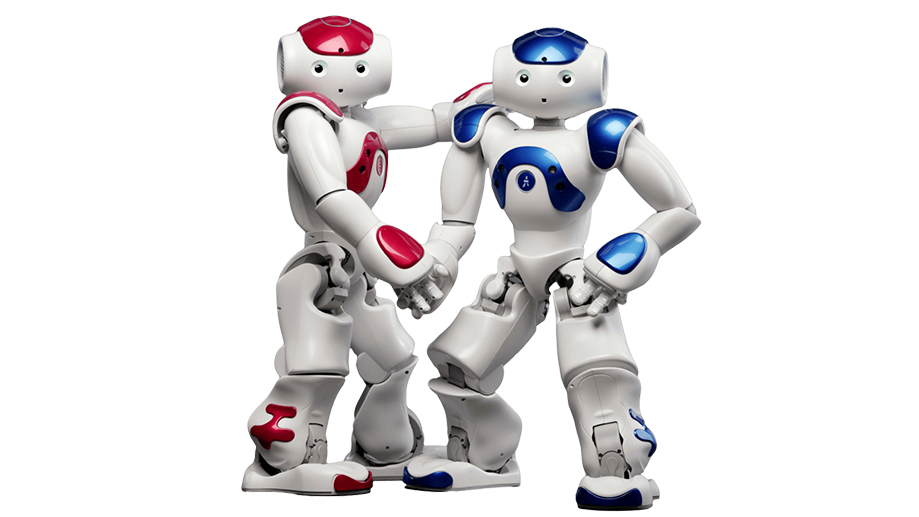
\includegraphics[height=5.5cm]{img/NAOIlustracion}
	\caption{Robot NAO en varios colores}
	\label{figura:NAOIlustracion}
\end{figure}

En esta hoja técnica \cite{NAOdatasheet} se detallan las características técnicas del robot que es objeto de estudio. Con unas dimensiones de 574x275x311mm y un peso de 5.4 kg, el robot consigue su movilidad mediante motores de corriente continua sin escobillas, siendo un total de 26 motores. En la imagen \ref{figura:NAOCinematica} podemos ver su esquema cinemático, en el cual se ven los ángulos de rotación y traslaciones. \\

\begin{figure}[!h]
	\centering
	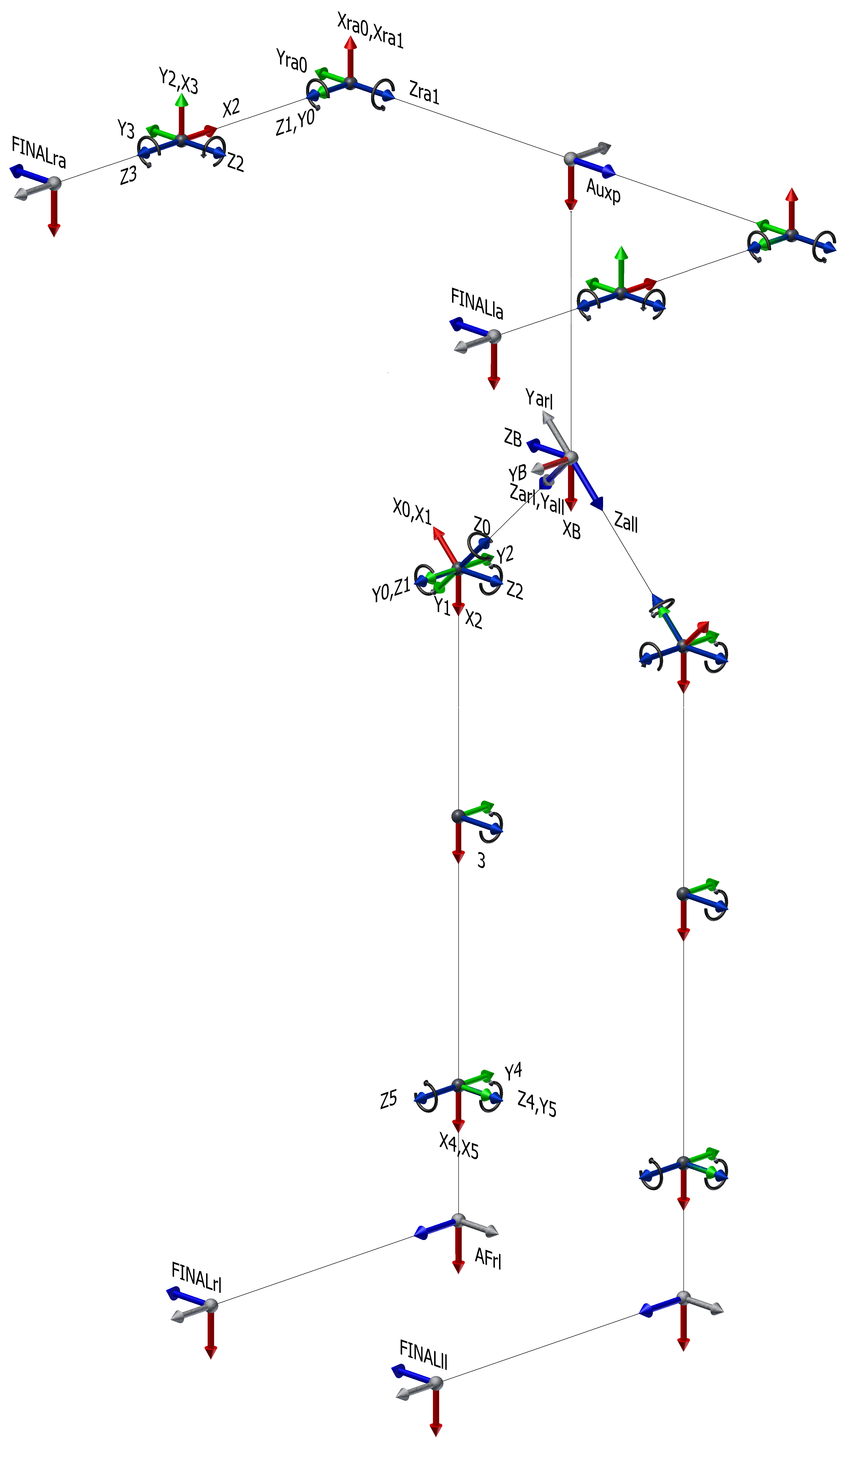
\includegraphics[height=10cm]{img/NAOCinematico}
	\caption{Esquema cinemático del robot NAO.}
	\label{figura:NAOCinematica}
\end{figure}

Como se ha mencionado antes, este proyecto parte de un proyecto anterior, cuyas limitaciones del propio robot suponen a su vez límites en el crecimiento de los procesos que lleva implementados. Precisamente, el componente que ejerce de tope es la unidad de cómputo y sus elementos asociados, como las memorias, o lo que el fabricante denomina \textit{Motherboard}. El límite es debido a que el robot incluye un simulador de diabetes que emplean librerías científicas. Esto supone un uso exhaustivo de los recursos de cómputo del robot, siendo que además del propio simulador, también corren otros procesos e hilos. Las características del robot para este aspecto podemos verlas en la tabla \ref{tabla:motherboardnao}: \\

\begin{table}[h]
\begin{center}
\begin{tabular}{|l|l|r|}
	\hline 
	\textbf{Elemento} & \textbf{Subelemento} & \textbf{Prestaciones} \\ 
	\hline 
	\textbf{CPU} & CPU Processor & Intel ATOM Z530 \\ 
	\hline 
	& Cache memory  & 512KB \\ 
	\hline 
	& Clock speed & 1.6GHz \\ 
	\hline 
	& FSB speed & 533MHz \\ 
	\hline 
	\textbf{RAM} &  & 1GB \\ 
	\hline 
	\textbf{Flash memory} &  & 2GB \\ 
	\hline 
	\textbf{Micro SDHC} &  & 8GB \\ 
	\hline 
\end{tabular} 
\caption{Motherboard del robot NAO}
\label{tabla:motherboardnao}
\end{center}
\end{table}

Para las aplicaciones de hoy en día, 1GB en memoria principal (RAM) es demasiado poco. Además teniendo en cuenta que aparte de ejecutar el código, que es muy cargante como se ha mencionado, también ejecuta otros procesos como por ejemplo la comunicación con sus actuadores y sensores mediante \textit{proxyes} como denomina el fabricante, o por ejemplo la comunicación via HTTP, SSH, entre otros. Por otra parte, el procesador Intel ATOM tienen un rendimiento bajo, como se muestra en a figura \ref{figura:IntelAtom}. No aparece el modelo de NAO, Atom Z530, pero el rendimiento es similar a los modelos que se muestran en la imagen. \\

\begin{figure}[!h]
	\centering
	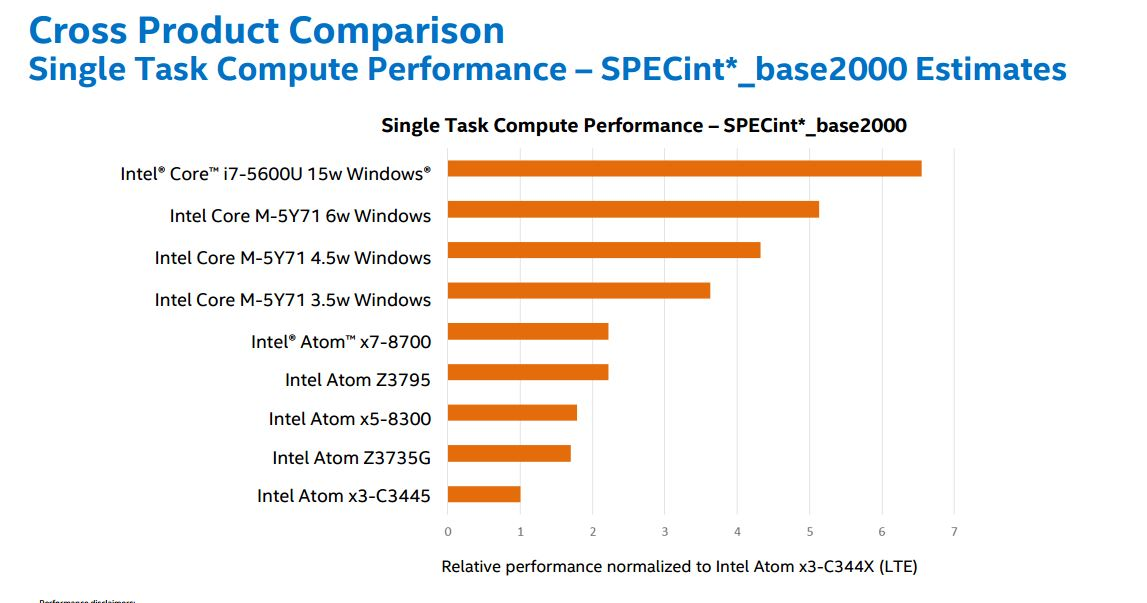
\includegraphics[height=7cm]{img/IntelAtom}
	\caption{Comparativa de rendimiento de procesadores Intel.}
	\label{figura:IntelAtom}
\end{figure}

Es importante entender que el modelo de comportamiento del páncreas que se sigue para simular la diabetes es el modelo \textbf{Hovorka}, cuya implementación puede encontrarse en sus documentos de investigación publicados, como por ejemplo \textbf{TODO: CITAR BIEN EL MODELO DE PANCREAS}. Su resolución pasa por ecuaciones diferenciales que se ejecutan periódicamente, lo cual resulta muy pesado para una máquina de las características que se han observado.

\section{Repaso del proyecto anterior}

El proyecto anterior estaba dividido en dos partes. La primera parte es la que actúa de \textbf{parte servidora} y se encuentra en el código del robot NAO. Mediante conexiones TCP, atiende peticiones de un cliente Java para obtener datos de la glucosa o para recibir órdenes. Contiene dentro cuatro hilos de ejecución, siendo el primero el hilo principal, que incluye un gestionador de hilos; el segundo el hilo que atiende las conexiones TCP; el tercero aloja el código del simulador, y por último, hay dos hilos excluyentes, es decir, que solamente puede haber uno activo cada vez. Estos son un hilo de escenario, que ejecuta el comportamiento de una persona con diabetes, atendiendo al estado de glucosa que tiene en un mismo instante y con funciones de inyectarse insulina. El otro hilo es un hilo de interacción, en el que solamente recibe órdenes sencillas y responde a ellas. \\

La otra parte del proyecto anterior es un \textbf{cliente Java}, el cual en el presente proyecto se va a dejar prácticamente intacto, pues solo va a sustituirse la parte del cliente TCP. Por lo demás, la interfaz solicita al servidor datos de glucosa actual al simulador de diabetes y envía órdenes al robot, que pueden ser acciones sobre los hilos o bien órdenes para que el robot ejecute movimientos o diga palabras.

\section{Objetivo}

El objetivo de este proyecto es \textbf{desengarzar la parte pesada del código del anterior proyecto para virtualizarla en un servicio en la nube}. Esta parte es el simulador de diabetes, que implementa ecuaciones muy costosas computacionalmente y emplea librerías científicas. \\

Esto implica una transformación total de la parte del código de NAO, que significa actualizar las partes del proyecto <<\textit{Desarrollo de un sistema de monitorización y control de un robot simulador de diabetes}>>. Se ha eliminado completamente TCP de la estructura del proyecto y se ha sustituido por MQTT o HTTP (REST), según necesidad. Las partes del proyecto por lo tanto necesitan estas modificaciones: 
\begin{itemize}
	\item Aplicación Java: En vez de utilizar una conexión TCP para conectarse al robot, deberá utilizar librerías para hacer llamadas HTTP y un cliente MQTT. 
	\item La parte de NAO: Sufre un cambio radical ya que se debe cambiar de C++ a Python 2.7 \textbf{TODO: RELACIONAR CON LA PARTE QUE LO JUSTIFICO}(la versión que admite NAO), y se divide el proyecto en dos partes:
		\subitem -- Google Cloud Engine: Se debe alquilar un servicio en la nube, en este caso del proveedor Google, y se montará un servidor que atenderá peticiones HTTP. Las responderá con el estado de la glucosa actualmente, ya que contendrá el simulador de diabetes.
		\subitem -- Código en NAO: Se debe eliminar toda la parte del simulador y TCP. Se añadirán dos librerías de HTTP y un cliente MQTT. 
\end{itemize}

\section{Estructura de la memoria}

Este proyecto se va a dividir en cuatro partes, que corresponden a las tres partes que conforman el proyecto y una cuarta sobre cómo se relacionan entre ellas. Las tres partes son las mencionadas en la sección anterior: Cliente Java, servicio en la nube y código en NAO. \\

Finalmente, se valorará el resultado del proyecto mediante unas conclusiones y se listarán una serie de posibles mejoras al proyecto actual. También hay un apéndice con información técnica acerca de cómo configurar los diferentes servicios.


\chapter{Servicio en la nube}

\section{Servicios en la nube actualmente}

Hoy en día existen empresas que ofrecen lo que se llama \textit{Cloud computing}, o lo que es lo mismo, computación en la nube o servicios en la nube, es un paradigma que permite ofrecer servicios de computación a través de una red, que usualmente es Internet. \\

La computación en la nube físicamente son servidores encargados de atender las peticiones recibidas en cualquier momento. Sirven a sus usuarios desde varios proveedores de alojamiento repartidos por todo el mundo. Este comportamiento está esquematizado en la figura \ref{figura:cloudcomputescheme}. Esta medida reduce los costos, garantiza un mejor tiempo de actividad y que los sitios web sean mucho más seguros. \\

\begin{figure}[!h]
	\centering
	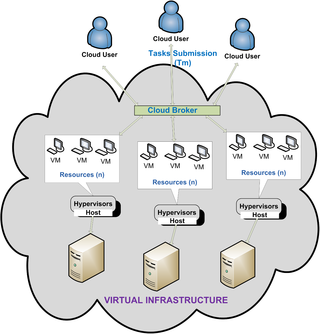
\includegraphics[height=7cm]{img/cloudcompute}
	\caption{Esquema de servicios en la nube.}
	\label{figura:cloudcomputescheme}
\end{figure}

Los servicios en la nube pueden ofrecer cierto nivel de servicios. Esto permite que, si se ofrece un nivel alto de servicio, el programador se ahorra tener que desarrollar la aplicación, pero la parte personalizable queda reducida. Por contra, si se contrata un nivel de servicio bajo, el programador deberá invertir tiempo en desarrollar la aplicación sobre el servicio y será mucho más personalizable. Estos tipos de nivel de servicio son:

\begin{itemize}
	\item \textbf{Iaas (Infraestructure as a Service)}: Permite gestionar al desarrollador aspectos como el sistema operativo, qué servidores quiere instalar en su máquina... Pero los aspectos hardware se hacen transparentes al programador. Un ejemplo de esto es el Google Compute Engine, ya que permite crear máquinas virtuales en las que se puede ejecutar cualquier tipo de software dentro.
	\item \textbf{Paas (Platform as a Service)}: Está un nivel por encima de IaaS, porque se hacen transparentes al programador, además de lo anterior, aspectos de sistema operativo, servicios de una máquina virtual... De manera que el desarrollador solamente debe rellenar algunas secciones de código. Un ejemplo de PaaS sería Google App Engine, ya que es una plataforma que permite redireccionar mediante peticiones REST aquellas peticiones a los fragmentos de código que ha escrito el programador.
	\item \textbf{Saas (Software as a Service)}: Cualquier servicio en la web listo para ser usado tal como está. Estos son los que los usuarios conocen más, porque son por ejemplo Google Drive, entre otros.
\end{itemize}

\begin{figure}[!h]
	\centering
	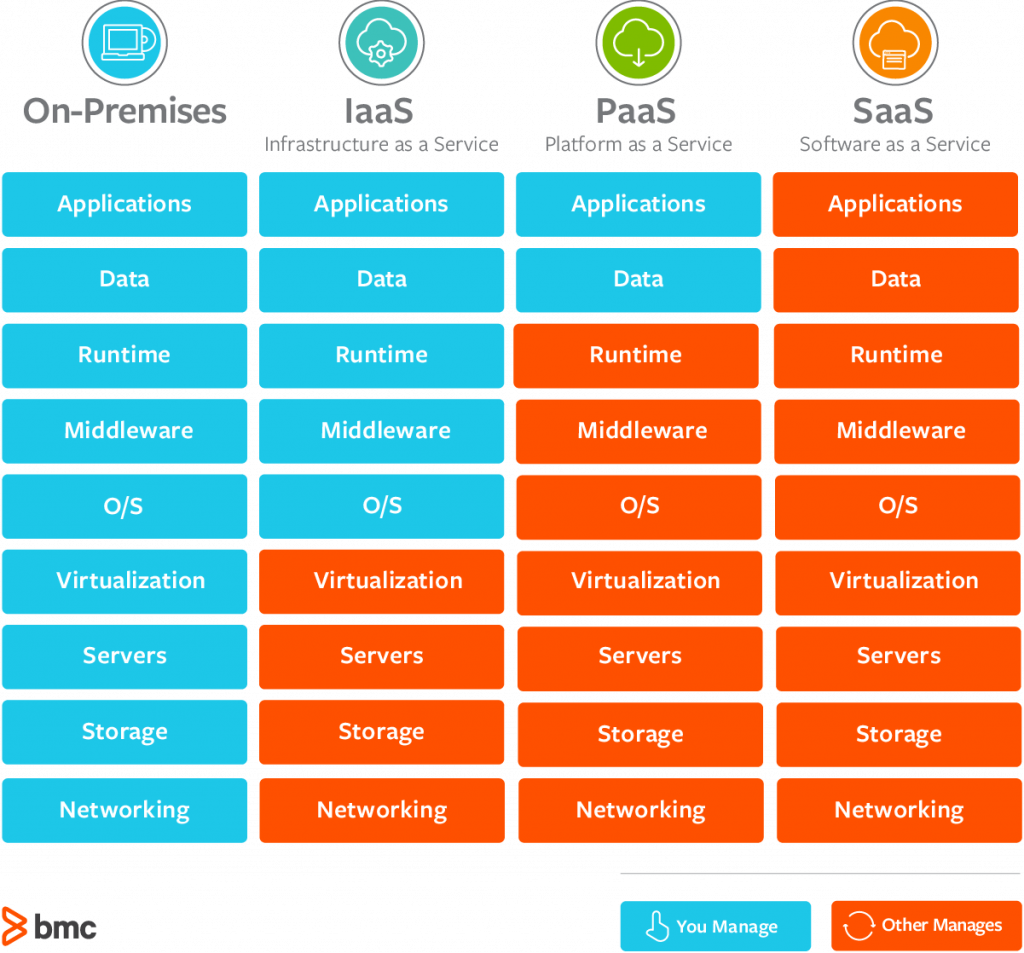
\includegraphics[height=7cm]{img/iaas_saas_paas}
	\caption{Niveles de servicio: IaaS, SaaS y PaaS.}
	\label{figura:IaasSaasPaas}
\end{figure}

En la figura \ref{figura:IaasSaasPaas} se aprecian las distintas capas que cubre cada uno de los niveles de servicio. Aparece uno no nombrado hasta ahora que es \textit{On-premises}; básicamente, se refiere a cómo serían los servicios localmente. \\

Hoy en día los mayores proveedores de servicios en la nube que existen son Amazon Web Services, IBM, Oracle, Alibaba, Google Cloud Services y Microsoft Azure. De las compañías mencionadas, las más grande y empleada en el mundo empresarial es Amazon Web Services, pero en este proyecto no se ha seleccionado debido a que la complejidad de su nube es muy alta, ya que ofrecen un total de 2400 aplicaciones como se indica en esta tabla \cite{ComparativaCloud}. Se ha escogido una más sencilla como es \textbf{Google Cloud Services}, que ocupa el tercer lugar y con una curva de aprendizaje mucho más rápida que sus anteriores. Además, el plan económico de Google Cloud Services es mucho más conveniente que otros. \\

\section{Google Cloud Services}

De la gama que ofrece Google Cloud Services, de la cual podemos ver una muestra en la imagen \ref{figura:googlecloudproducts} se han estado contemplando varias opciones. En un primer lugar, se estuvo barajando trabajar con Google App Engine, que como se ha nombrado antes, es un PaaS. Así, el trabajo a realizar se consideraría notablemente. Pero tuvo que descartarse debido a que ciertas partes como la concurrencia de hilos no eran compatibles con el diseño del PaaS. Se estuvieron mirando otros productos para complementarlo, como son Google Tasks o Google Cloud Storage, pero la combinación no podían generar un servicio de simulación de diabetes en la nube, como era el propósito. Para tener más libertad, se ha escogido para este proyecto un \textbf{IaaS}, \textbf{Google Compute Engine}, porque tiene mucha flexibilidad para programar los servicios que se deseen. \\

\begin{figure}[!h]
	\centering
	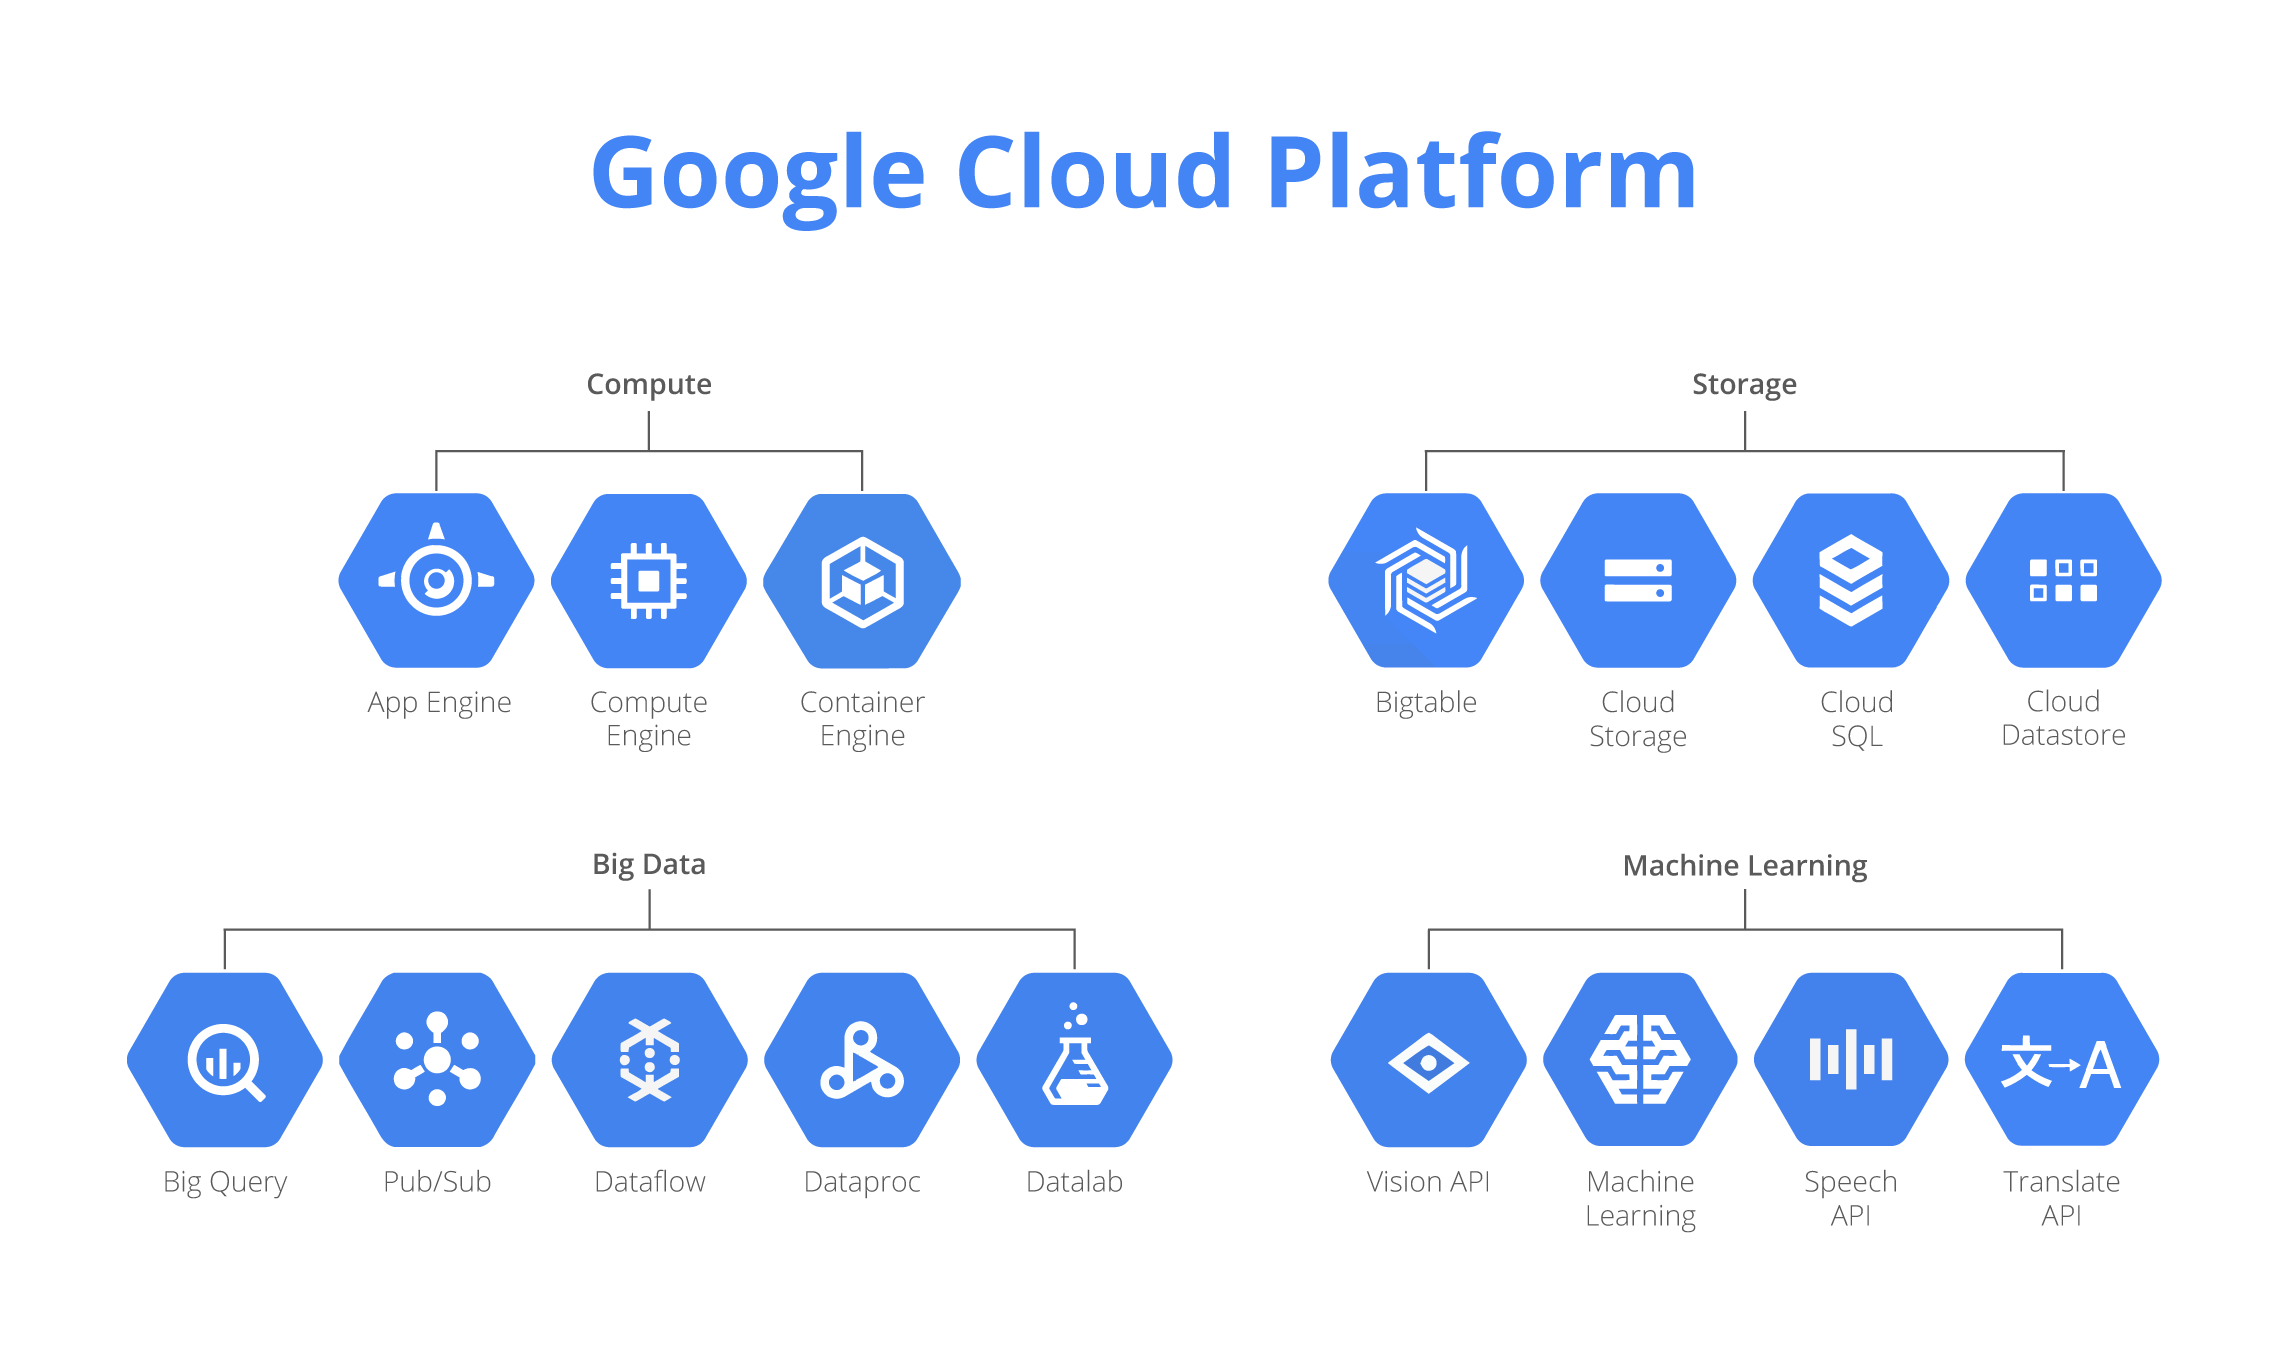
\includegraphics[height=8cm]{img/googlecloudproducts}
	\caption{Productos de Google Cloud.}
	\label{figura:googlecloudproducts}
\end{figure}

Google Compute Engine, o GCE es básicamente una infraestructura que permite levantar \textbf{máquinas virtuales} de forma escalable a las cuales se puede acceder via SSH, API, y más formas. Esta máquina virtual, a la hora de crearla, deja escoger qué tipo de memoria principal tiene, el sistema operativo y el número de CPUs (\textit{Central Processing Unit}) y TPUs (\textit{Tensor Processing Unit}); este último componente se emplea para los mecanismos de aprendizaje automático, que en este caso no aplica.

Como se menciona en la tabla \ref{tabla:caracteristicasgce}, en la cual podemos ver las características de la máquina virtual empleada para contener el simulador de diabetes, la IP es necesario que sea estática; se necesita que tanto el robot como la aplicación Java sepan dónde se encuentra el servicio en la nube en todo momento. \\

\begin{table}[!h]
	\begin{center}
		\begin{tabular}{|l|r|}
			\hline 
			\textbf{Característica} & \textbf{Descripción} \\ 
			\hline 
			Sistema operativo & Ubuntu 19.04 \\ 
			\hline 
			Memoria principal & 3,75 GB \\ 
			\hline 
			Memoria del disco & 10 GB \\ 
			\hline 
			CPU & 1 vCPU \\ 
			\hline 
			IP & Estática (34.76.240.69) \\ 
			\hline 
		\end{tabular} 
		\caption{Características de la máquina virtual de GCE}
		\label{tabla:caracteristicasgce}
	\end{center}
\end{table}

Se han levantado dos servicios dentro de la máquina virtual, para cada uno de los cuales debe entrarse por un puerto diferente. El primero es un \textit{broker} MQTT, el cual se explica en la sección  y el segundo el propio servidor para el simulador de diabetes. \\

\section{Servidor de diabetes}

Del proyecto anterior, se ha quitado la parte del simulador de diabetes y se ha movido a la máquina virtual de Google Compute Engine, como se ha comentado en otras secciones. Pero para acceder a él y poder manejarlo, antes debe superponerse una capa (API, \textit{Application Programming Interface}) para el manejo de peticiones entrantes. En este caso se ha decidido utilizar el modelo REST sobre un servidor HTTP.

\subsection{HTTP}
HTTP, o \textit{HyperText Transfer Protocol}, es el protocolo de red que permite la transferencia de documentos de hipermedia en la red, generalmente entre un navegador y un servidor aunque en este proyecto sea a través de una aplicación Python y Java, para que los humanos puedan leerlos. \\

Sobre las URLs de los servicios web se pueden hacer muchos tipos de operaciones, que son exactamente: GET, HEAD, POST, PUT, DELETE, TRACE, OPTIONS, CONNECT, PATCH, SEARCH, COPY, LOCK, UNLOCK, MOVE, MKCOL, PROPFIND, PROPPATCH, MERGE, UPDATE y LABEL. Se aprecia que los nombres son cuasi descriptivos por si solos. \\

Las peticiones y las respuestas de peticiones llevan una cabecera con metadatos para indicar por ejemplo si lo que va a recibirse está en formato XML, JSON... (Se llama MimeType), o el lenguaje de la respuesta, entre otras opciones de metadatos. Después de las cabeceras viene el cuerpo del mensaje en sí, que contiene la información solicitada o de petición. \\

También está en el protocolo el código de las respuestas. Según el código recibido quieren decir una cosa u otra, pero se agrupan en cinco tipos de formato de código:
\begin{itemize}
	\item Formato 1xx: Respuestas informativas. Indica que la petición ha sido recibida y se está procesando.
	\item Formato 2xx: Respuestas correctas. Es el resultado deseado.
	\item Formato 3xx: Respuestas de redirección. Indica que el cliente necesita realizar más acciones para finalizar la petición.
	\item Formato 4xx: Errores causados por el cliente. Indica que ha habido un error en el procesado de la petición a causa de que el cliente ha hecho algo mal.
	\item Formato 5xx: Errores causados por el servidor. Indica que ha habido un error en el procesado de la petición a causa de un fallo en el servidor.
\end{itemize}

\subsection{REST}
Como se menciona en este artículo \cite{PrincipiosREST}, REST fue presentado por primera vez en el 2000 por Roy Fielding en la Universidad de California. REST (\textit{Representational State Transfer}) es una arquitectura de programación pensada para servicios web, que se transfieren mediante HTTP. Ha desplazado enormemente a SOAP gracias a su sencillez de uso y de entendimiento. Sigue cuatro principios de diseño:
\begin{itemize}
	\item Utilice métodos HTTP de forma explícita: El cliente interactúa con el servidor únicamente con métodos HTTP mediante operaciones de crear, leer, actualizar y borrar, que para REST son:
		\subitem -- Para crear un recurso en el servidor hay que utilizar un POST.
		\subitem -- Para consultar un recurso hay que utilizar un GET.
		\subitem -- Para cambiar el estado de un recurso hay que utilizar un PUT.
		\subitem -- Para borrar un recurso hay que utilizar un DELETE.
	\item Sea sin estados: Un mensaje no tiene porqué depender de un mensaje anterior para que se entienda, sino que cada mensaje debe tener toda la información necesaria.
	\item Exponga los URIs (\textit{Uniform Resource Identifier}) como estructuras de directorios. 
	\item Transfiera XML, JavaScript Object Notation (JSON), o ambos.
\end{itemize}

\subsection{HTTP y REST en este proyecto}
Se ha decidido emplear HTTP y REST en este proyecto porque como se mencionaba antes, su uso es el más extendido hoy en día debido a su sencillez. \\

Como se aprecia, HTTP y REST por si solos no pueden entenderse, pues HTTP necesita guiarse por el patrón que marca REST y REST necesita que HTTP de cuerpo a su arquitectura. Así que se explican de manera conjunta. \\

Se ha seguido la estructura de las URIs como REST manda que se monte, es decir, como una estructura de directorios. Cuando se compone toda la URL, y se implementan los métodos, los puntos de acceso al servidor y sus respuestas son los que se indican en las tablas \ref{tabla:urishttpget} y \ref{tabla:urishttpput}. En esta tabla se ha recortado la URL y se ha dejado solamente la ruta hasta el recurso. La URL absoluta tiene el prefijo \url{http://34.76.240.69:8080}, que por ejemplo para acceder al recurso raíz (/) será \url{http://34.76.240.69:8080/}, o para acceder a /Hilo/, \url{http://34.76.240.69:8080/Hilo/}. Nótese que solamente se han empleado los métodos HTTP GET y PUT, pues solo se permiten operaciones de lectura y de actualización de recursos.

\begin{table}[!h]
\begin{center}
\begin{tabular}{|l|c|c|}
	\hline 
	\textbf{URL} & \textbf{GET} & \textbf{Respuesta}\\ 
	\hline 
	/ & Sí & Es para probar la conectividad, \\ 
	&& devuelve "Hello World".\\
	\hline 
	/Hilo/ & Sí & Devuelve el estado del hilo:\\ 
	&& PARADO, PAUSADO, CORRIENDO. \\
	\hline 
	/Simulador/Modo/ & Sí & Devuelve el modo actual del simulador.\\ 
	\hline 
	/Simulador/Glucosa/ & Sí & Devuelve la glucosa actual\\ 
	&& del simulador de diabetes.\\
	\hline 
	/Simulador/ & Sí & Devuelve, si lo tiene, el dato\\ 
	DatosSimulacion/&& de simulación que se ha enviado.\\
	\hline 
\end{tabular} 
\caption{Estructura de URIs y descripción de método HTTP GET sobre el servidor de diabetes.}
\label{tabla:urishttpget}
\end{center}
\end{table}

\begin{table}[!h]
	\begin{center}
		\begin{tabular}{|l|c|c|}
			\hline 
			\textbf{URL} & \textbf{PUT} & \textbf{Respuesta} \\ 
			\hline 
			/ & No & - \\ 
			\hline 
			/Hilo/ & Sí, acepta como & Si se ha podido aplicar  \\ 
			& parámetros PARADO, & la operación al hilo,\\
			& PAUSADO, CORRIENDO. & devuelve 200 OK,\\
			& sino respuesta 4xx. & \\
			\hline 
			/Simulador/Modo/ & Sí, admite los valores 1,2,3 & Si todo ha ido bien,\\ 
			&& 200 OK, sino 4xx. \\
			\hline 
			/Simulador/Glucosa/ & No & - \\ 
			\hline 
			/Simulador/ & Sí, admite un JSON & Si todo ha ido bien, \\ 
			DatosSimulacion/ & con los datos para & 200 OK, sino 4xx.\\
			& una nueva simulación. & \\
			\hline 
		\end{tabular} 
		\caption{Estructura de URIs y descripción de método HTTP PUT sobre el servidor de diabetes.}
		\label{tabla:urishttpput}
	\end{center}
\end{table}

Para hacer real esta estructura, esta \textit{API}, hay que programarlo en alguna tecnología. Se escoge \textbf{Python 2.7}, para mantener la coherencia con el resto del proyecto, el código en NAO, que está obligado a ser en Python 2.7 también, como se explica más adelante. Antes estaba escrito en C++, pero existen utilidades más modernas y moldeables en Python, por lo que se aprovecha el gran cambio que va a sufrir el simulador para convertirlo a un lenguaje más flexible. \\

Primero, se utiliza un \textbf{servidor WSGI en el puerto 8080} para que la aplicación Python escuche las peticiones entrantes. WSGI significa \textit{Web Server Gateway Interface} y es el conjunto de servidores web que reenvían las peticiones a las aplicaciones web escritas en Python. Tienen dos partes: la primera la parte del servidor en si, que en este caso está construida sobre Nginx, y la segunda, que es la implementación de la API REST en sí. De las posibles opciones que existen en Python, se ha escogido \textbf{gevent}, cuyo sitio oficial se encuentra en \cite{WSGIGevent}. Crear una aplicación web con WSGI es muy sencillo y más aún si se combina con Flask. \\

\textbf{Flask} es un \textit{web framework}, lo que significa un conjunto de herramientas y librerías que hacen muy simple estructurar una aplicación web. Su mayor competidor es Django, pero es más recomendable utilizar Flask junto con Python, por no mencionar que es mucho más simple utilizar Flask. Dado que la API construida no tiene más que un dos clientes, tampoco es necesario algo muy potente, así que la simpleza se valora más. Añadido a Flask, hay una extensión llamada \textbf{Flask RESTful} \cite{FlaskRESTful} que abstrae un método Flask convencional para convertirlo en una serie de operaciones sobre un recurso de la jerarquía de URIs.\\

Juntando la máquina de Google Compute Engine y las tecnologías para montar la API REST --WSGI y Flask--, se consigue hacer la puerta de entrada para poder interactuar con el simulador, el cual está encapsulado en un hilo de ejecución. Mediante la API REST se puede activar, pausar, detener o reanudar la ejecución del hilo de ejecución del simulador, así como consultar la glucosa actual en cada momento o enviar datos para simular. Pero lo que falta por convertir es la librería que hace el cálculo de las ecuaciones diferenciales.

\section{MQTT}

\subsection{Introducción a MQTT}

MQTT significa \textit{Message Queue Telemetry Transport}. Es un protocolo del tipo publicador/suscriptor, extremadamente simple y ligero, diseñado para dispositivos limitados o con poco ancho de banda. Los principios de diseño son minimizar el ancho de banda de la red y los requisitos de recursos del dispositivo al mismo tiempo que se intenta garantizar la confiabilidad y cierto grado de garantía de entrega. Estos principios también hacen que el protocolo sea ideal para el emergente mundo de dispositivos conectados <<máquina a máquina>> (M2M) o <<Internet de las cosas>> (IoT), y para aplicaciones móviles donde el ancho de banda y la energía de la batería son muy importantes. Además, la versión 3.1.1 se encuentra certificada en la ISO/IEC PRF 20922 \cite{MQTTISO}. \\

En MQTT hay dos tipos de agentes que intervienen: 
\begin{itemize}
	\item El \textbf{\textit{broker}}: Es el servidor que contiene las colas de mensajes. Los clientes depositan mensajes en las colas (\textit{publican} estos mensajes) de forma que otros clientes reciben estos mensajes encolados. Solo existe un broker por cada sistema MQTT.
	\item \textbf{Clientes}: Puede haber tantos clientes como se desee. Son los que generan los mensajes que envían al broker, y el broker se encarga de distribuirlos a los clientes que pertoque. 
\end{itemize}

El hecho de enviar un mensaje al broker se llama \textbf{publicar}, y para que un cliente pueda recibir los mensajes, debe \textbf{estar suscrito} a ellos. La operación de recepción de un mensaje es asíncrona, pues se reciben los mensajes y se ejecuta una llamada como consecuencia (\textit{callback}). Para identificar a qué suscriptores pertenece cada mensaje, se emplean unas etiquetas, que pueden contener niveles de jerarquía, al estilo de los directorios en sistemas operativos. Por ejemplo, si se publica un mensaje \textit{topic1/topic2}, y un suscriptor indica que desea recibir los mensajes sobre esa etiqueta, así se hará. Pero hay dos carácteres especiales. Supóngase la etiqueta de ejemplo anterior: 
\begin{itemize}
	\item \textbf{\#}: Si un cliente decide suscribirse a \textit{topic1/\#}, recibirá todos los mensajes cuya etiqueta comience por \textit{topic1/}.
	\item \textbf{+}: Si algún suscriptor decide suscribirse a \textit{+/topic2}, recibirá todos aquellos mensajes que comiencen por cualquier etiqueta en el primer nivel, pero que en el segundo nivel se llamen \textit{topic2}.
\end{itemize} 

Puede observarse un ejemplo gráficamente en la figura \ref{figura:mqttexplanation}.

\begin{figure}[!h]
	\centering
	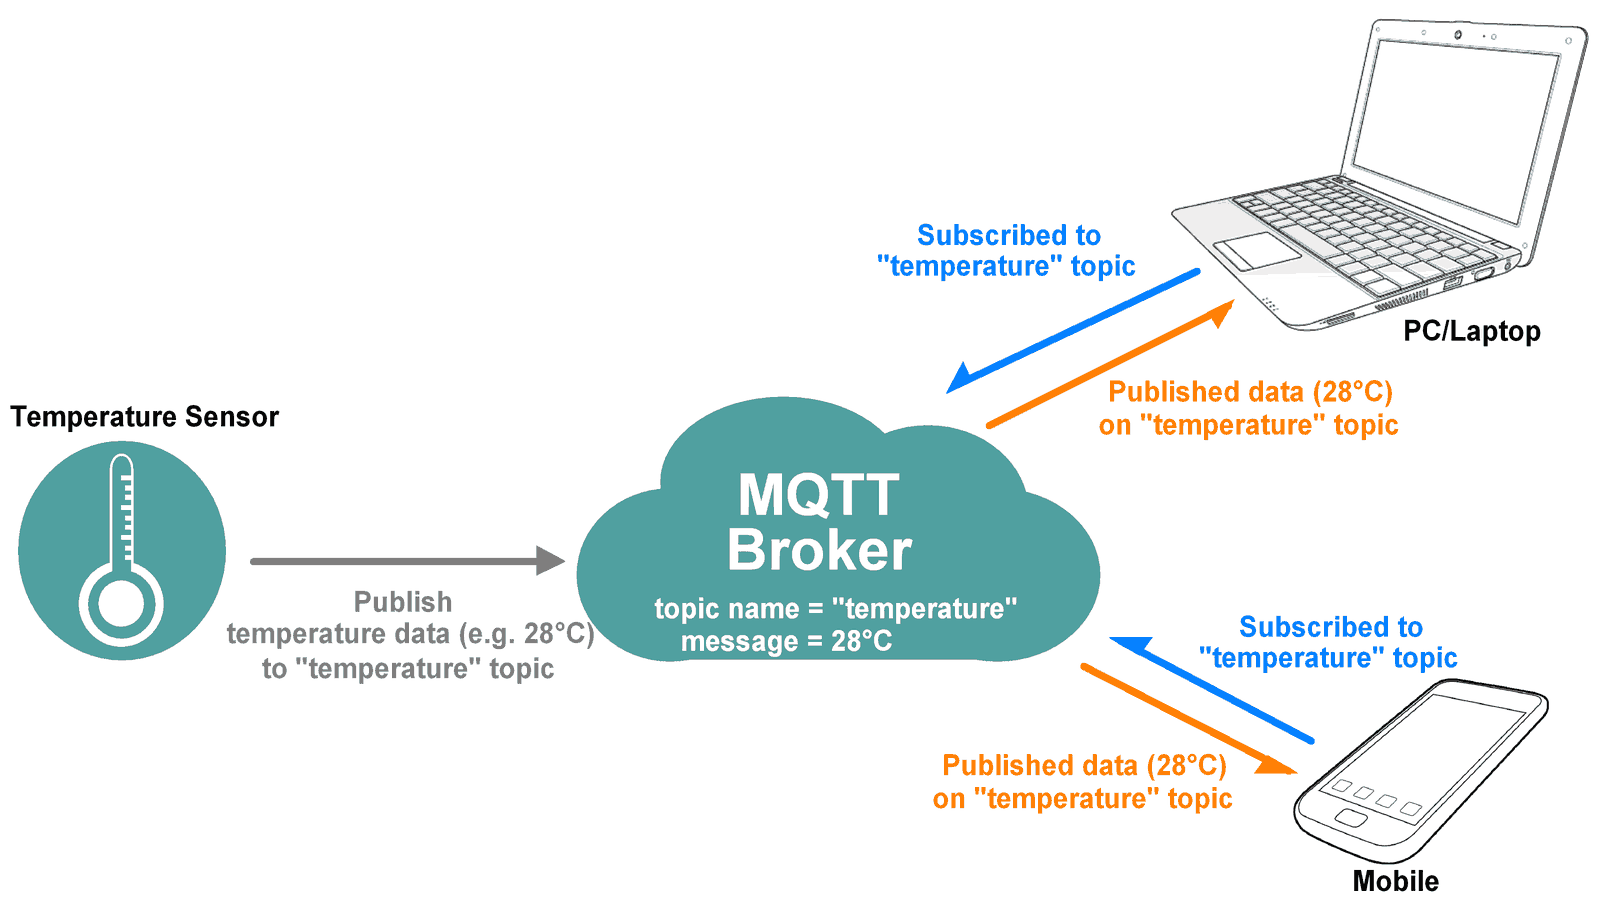
\includegraphics[height=8cm]{img/mqttexplanation}
	\caption{Ejemplo del funcionamiento de MQTT.}
	\label{figura:mqttexplanation}
\end{figure}

Existen muchas implementaciones de MQTT: Paho MQTT, Mosquitto, HiveMQ, Adafruit IO, las cuales son las más famosas, pero hay más. Muchas de ellas son de código abierto, otras no, están desarrolladas por diversas empresas o universidades y demás características que se pueden observar en este enlace \cite{MQTTComparison}. \\

\subsection{MQTT en este proyecto}

Para este proyecto se han empleado dos tipos de MQTT del mismo proveedor, Eclipse, que ha desarrollado M2Mqtt, Mosquitto y Paho MQTT. El primero, \textbf{Mosquitto}, se ha utilizado para instalar el \textbf{broker} en la máquina virtual. Dado que Mosquitto es la única de las tres implementaciones de Eclipse que tiene un broker, no había más opción que instalarlo. Para cliente, solamente tiene integración con el lenguaje de programación C, así que se desarrollan los \textbf{clientes} con \textbf{Paho MQTT}, que es el segundo componente, pues tiene un nivel de compatibilidad muy alto -- se adapta a C, C++, Java, JavaScript, Python y Go. \\

Dado que el broker Mosquitto se implementa en la máquina virtual, que lleva Ubuntu 19.04 como sistema operativo, la fuente de instalación es los propios repositorios de Ubuntu. Se instala sobre el puerto \textbf{TCP 1883} y se emplea autenticación de usuario y contraseña. La conexión es no-TLS (\textit{Transport Layer Security}), pero si se quisiera una conexión cifrada (TLS) debería instalarse en el puerto 8883. Para activar el servidor no hay que hacer más que activar un servicio con \textit{systemctl}. \\

Los clientes MQTT están tanto en el código NAO como en la aplicación Java, y ambos tienen detallados su funcionamiento en sus secciones pertinentes. \\

La intención para este sistema es sustituir la conexión TCP que enviaba mensajes periódicamente por una conexión asíncrona como es ésta, mucho más ligera a nivel computacional. Se envían mensajes para el arranque de hilos, órdenes directas al robot, mensajes de estado, entre otros.

\section{Librería para el cálculo diferencial}

Lo último necesario para terminar de migrar el simulador de diabetes a una aplicación web Python es adaptar la librería de cálculo diferencial. Tal como se menciona en la introducción de este proyecto, se sigue un modelo de simulación según Hovorka que emplea ecuaciones ODE (ecuaciones diferenciales ordinarias). En el simulador del anterior proyecto se emplea la librería Alglib, hecha para C++. Al convertir la aplicación a Python, es necesario cambiar también la librería de cálculo. \\

Alglib \cite{Alglib} tiene una licencia comercial y otra gratuita, esta última para fines no comerciales como es esta aplicación. Empleando la opción gratuita, existe un \textit{wrapper} o una aplicación que engloba a la librería construida para C++, para que pueda utilizarse en Python. En un principio se había pensado en emplear esta opción para respetar los cálculos iniciales pero supone una limitación a la hora de actualizar la librería de la aplicación Python. Esta librería para actualizarse depende de que se actualice su código interno C++ y luego el \textit{wrapper} para ésta. \\

Por lo tanto se ha migrado la librería de cálculo a \textbf{SciPy} \cite{Scipy}, un módulo Python para cálculo matemático entre otras funciones, cuyo uso está muy extendido. De hecho, de sus paquetes centrales, existen unos que son muy famosos como NumPy, IPython o Matplotlib.

\chapter{Código en NAO}

Idees de estructura:
- Explicació del NAO i tipos de llenguatge
- Explicació del projecte anterior i arquitectura (dibuixets de TCP)
- Explicació de les limitacions de còmput de NAO i de limitacions de TCP
- Estructura del meu projecte. MQTT entrar en detall del QoS. (Part Java, Part NAO i part GCloud).
- Part Java: Mínim canvi realment. Explicar Paho i que es un client Rest.
- Part NAO: Que he reconvertit el codi a Python perquè el NAO te molt mal el C++. 
- Part GCloud: Aquí explayar-se.
- Millores: Prescindir de GCloud i montarse una raspi amb un DNS, afegir més funcions al NAO, mes precisio del simulador aprofitant gcloud, manejar varios NAOs amb una sola app java i un sol gcloud...

\chapter{Aplicación Java}

????? ????????????? ????????????? ????????????? ????????????? ?????????????

\chapter{Relación entre los componentes}

????? ????????????? ????????????? ????????????? ????????????? ????????????? 

\section{?? ???? ???? ? ?? ??}

????? ????????????? ????????????? ????????????? ????????????? ?????????????

%%%%%%%%%%%%%%%%%%%%%%%%%%%%%%%%%%%%%%%%%%%%%%%%%%%%%%%%%%%%%%%%%%%%%%%%%%%%%%%
%                                 CONCLUSIONS                                 %
%%%%%%%%%%%%%%%%%%%%%%%%%%%%%%%%%%%%%%%%%%%%%%%%%%%%%%%%%%%%%%%%%%%%%%%%%%%%%%%

\chapter{Conclusions}

\section{Mejoras} 

Poder arrancar la MV desde API \\
Hacer la app Java una app web en el GCE \\
Controlar mas de un robot con su simulador asignado a la vez

\section{Conclusiones}

?????????????????????????????????????

%%%%%%%%%%%%%%%%%%%%%%%%%%%%%%%%%%%%%%%%%%%%%%%%%%%%%%%%%%%%%%%%%%%%%%%%%%%%%%%
%                                BIBLIOGRAFIA                                 %
%%%%%%%%%%%%%%%%%%%%%%%%%%%%%%%%%%%%%%%%%%%%%%%%%%%%%%%%%%%%%%%%%%%%%%%%%%%%%%%

\begin{thebibliography}{10}

%%%%%%%%%%%%%%%%%%%%%%%%%%%%%%%%%%%%%%%%%%%%%%%%%%%%%%%%%%%%%%%%%%%%%%%%%%%%%%%
% MODEL D'URL                                                                 %
%%%%%%%%%%%%%%%%%%%%%%%%%%%%%%%%%%%%%%%%%%%%%%%%%%%%%%%%%%%%%%%%%%%%%%%%%%%%%%%
\bibitem{NAOWiki}
   Breve explicación de qué es el robot NAO. \\
   \newblock Consultado en: \\ 
   \url{https://es.wikipedia.org/wiki/Nao_(robot)}
   
\bibitem{NAOdatasheet}
	Características técnicas del Robot NAO. \\
	\newblock Consultado en: \\
   	\url{https://static1.squarespace.com/static/52e733d8e4b062fc0c603ea8/t/53a13620e4b0d80b1acadb20/1403074080427/nao_datasheet.pdf}

\bibitem{TFMAnterior}
	Desarrollo de un sistema de monitorización y control de un robot simulador de diabetes. Autor: Antonio Bengochea Carrasco. \\
	\newblock Consultado en: \\
	\url{https://riunet.upv.es/bitstream/handle/10251/94065/BENGOCHEA\%20-\%20Desarrollo\%20de\%20un\%20sistema\%20de\%20monitorizaci\%C3\%B3n\%20y\%20control\%20de\%20un\%20robot\%20simulador\%20de\%20diabetes.pdf?sequence=3}
	
\bibitem{ComparativaCloud}
	Cuadro comparativo con las empresas de Cloud Computing \\
	\newblock Consultado en: \\
	\url{https://recursos.apser.es/hubfs/Infograf\%C3\%ADas/APS-Cuadro-comparativo-grandes-cloud.pdf}
	
\bibitem{MQTT}
	Información sobre MQTT \\
	\newblock Consultado en: \\
	\url{http://mqtt.org/}
	
\bibitem{MQTTISO}
	ISO sobre MQTT v3.1.1 \\
	\newblock Consultado en: \\
	\url{https://www.iso.org/standard/69466.html}
	
\bibitem{MQTTComparison}
	Comparación de las implementaciones de MQTT \\
	\newblock Consultado en: \\
	\url{https://en.wikipedia.org/wiki/Comparison_of_MQTT_implementations}

\bibitem{PrincipiosHTTP}
	Principios de HTTP \\
	\newblock Consultado en: \\
	\url{https://es.wikipedia.org/wiki/Protocolo_de_transferencia_de_hipertexto}
	
\bibitem{WSGIGevent}
	WSGI de Gevent \\
	\newblock Consultado en: \\
	\url{http://www.gevent.org/}
	
\bibitem{PrincipiosREST}
	Principios de servicios RESTful \\
	\newblock Consultado en: \\
	\url{https://www.ibm.com/developerworks/ssa/library/ws-restful/index.html}
	
\bibitem{Flask}
	¿Por qué es Flask una buena elección para web? \\
	\newblock Consultado en: \\
	\url{https://www.fullstackpython.com/flask.html}
	
\bibitem{FlaskRESTful}
	Manual de la extensión de Flask para REST \\
	\newblock Consultado en: \\
	\url{https://flask-restful.readthedocs.io/en/latest/}
	
\bibitem{Alglib}
	Página principal de Alglib \\
	\newblock Consultado en: \\
	\url{http://www.alglib.net/}
	
\bibitem{Scipy}
	Página principal de la librería SciPy\\
	\newblock Consultado en: \\
	\url{https://www.scipy.org/}
	

\end{thebibliography}
\cleardoublepage

%%%%%%%%%%%%%%%%%%%%%%%%%%%%%%%%%%%%%%%%%%%%%%%%%%%%%%%%%%%%%%%%%%%%%%%%%%%%%%%
%                           APÈNDIXS  (Si n'hi ha!)                           %
%%%%%%%%%%%%%%%%%%%%%%%%%%%%%%%%%%%%%%%%%%%%%%%%%%%%%%%%%%%%%%%%%%%%%%%%%%%%%%%

\APPENDIX

%%%%%%%%%%%%%%%%%%%%%%%%%%%%%%%%%%%%%%%%%%%%%%%%%%%%%%%%%%%%%%%%%%%%%%%%%%%%%%%
%                         LA CONFIGURACIO DEL SISTEMA                         %
%%%%%%%%%%%%%%%%%%%%%%%%%%%%%%%%%%%%%%%%%%%%%%%%%%%%%%%%%%%%%%%%%%%%%%%%%%%%%%%

\chapter{Configuració del sistema}

????? ????????????? ????????????? ????????????? ????????????? ?????????????

\section{Fase d'inicialització}

????? ????????????? ????????????? ????????????? ????????????? ?????????????

\section{Identificació de dispositius}

????? ????????????? ????????????? ????????????? ????????????? ?????????????

%%%%%%%%%%%%%%%%%%%%%%%%%%%%%%%%%%%%%%%%%%%%%%%%%%%%%%%%%%%%%%%%%%%%%%%%%%%%%%%
%                               ALTRES  APÈNDIXS                              %
%%%%%%%%%%%%%%%%%%%%%%%%%%%%%%%%%%%%%%%%%%%%%%%%%%%%%%%%%%%%%%%%%%%%%%%%%%%%%%%


\chapter{??? ???????????? ????}

????? ????????????? ????????????? ????????????? ????????????? ????????????? 



%%%%%%%%%%%%%%%%%%%%%%%%%%%%%%%%%%%%%%%%%%%%%%%%%%%%%%%%%%%%%%%%%%%%%%%%%%%%%%%
%                              FI DEL DOCUMENT                                %
%%%%%%%%%%%%%%%%%%%%%%%%%%%%%%%%%%%%%%%%%%%%%%%%%%%%%%%%%%%%%%%%%%%%%%%%%%%%%%%

\end{document}
